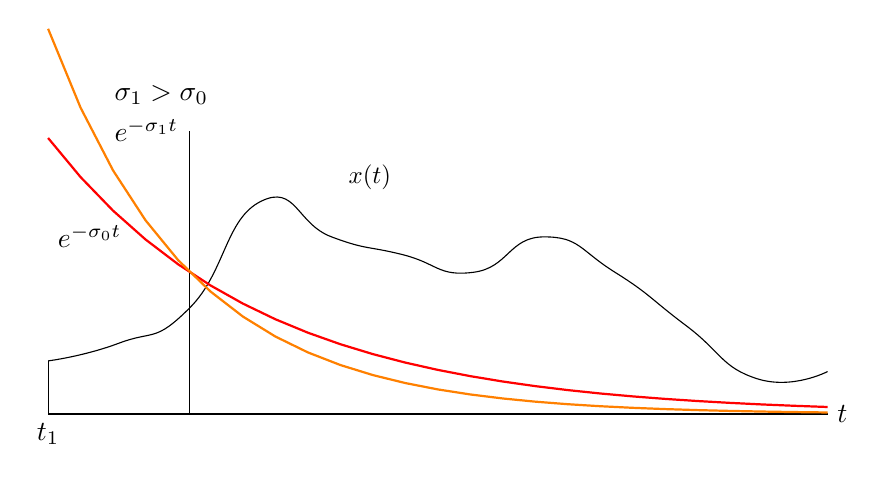
\begin{tikzpicture}[scale=0.9]
\draw (-2,0) -- (9,0) node[anchor=west] {$t$};
\draw (0,0) -- (0, 4);
\draw  plot[smooth, tension=0.9] coordinates {(-2, 0.75) (-1,1) (0,1.5)(1,3) (2,2.5) (3,2.25) (4,2) (5,2.5) (6,2) (7,1.25) (8,0.5) (9, 0.6)} node[midway, anchor=south, yshift=1.2in, xshift=1in] {$x(t)$};
\draw (-2, 0.75) -- (-2, 0) node[anchor=north] {$t_1$}  ;
\onslide<2->
{
\draw[thick, red,domain=0:11] plot({\x-2},{2*exp(-(\x-2)/3)}) ;

    \node at (-2, 2.5)  [anchor=west] {$e^{-\sigma_0 t}$};
}
\onslide<3->
{

  \draw[thick, orange,domain=0:11] plot({\x-2},{2*exp(-(\x-2)/2)});
\node at   (-1.2,4)  [anchor=west] {$e^{-\sigma_1 t}$};
    \node at (-1.2, 4.5) [anchor=west] {$\sigma_1>\sigma_0$};
}
\end{tikzpicture} 